\documentclass[aps,prd,preprint,notitlepage,nofootinbib]{revtex4-2}
\usepackage{amsmath,amssymb,booktabs,tabularx,graphicx,hyperref}
\setlength{\emergencystretch}{3em}
\Urlmuskip=0mu plus 2mu\relax
\hypersetup{colorlinks=true,urlcolor=blue}
\begin{document}
\title{Spinning and Boosted Trumpet Initial Data:\\Formulation and Validation Status}
\author{TwoPuncturesC and AthenaK integration}
\date{18 October 2026 --- interim report}
\begin{abstract}
We implement quasi-isotropic (QI), $R_0=M$ trumpet and Liu wormhole seeds
with portable AthenaK import. First Cartesian focus compatibility reduces
the finest moderate QI bulk momentum RMS by 21.9 to $7.77\times10^{-9}$.
\textbf{The strict bulk-convergence gate remains failed.} One fixed
three-grid formulation meets absolute physical constraint bounds; a
calibrated sixth-order observer confirms the residual rise. Stronger second
compatibility worsens the error and is rejected. Finest-grid AthenaK horizons
pass angular, quadrature and interior-enclosure checks. Matched-count
Bowen--York Hamiltonian RMS is near $10^{-10}$, at the observer calibration
floor; failed native stopping gates are retained. Isolated Liu $\chi=0.99$
controls pass; direct spherical Liu data now converge at $\chi=0.9999$. Lower-resolution QI data converge before the high-grid bulk issue appears. Moderate trumpet and extreme binaries remain unqualified.
\end{abstract}
\maketitle

\section{Construction and its limits}
The reference is the $R_0=M$ stationary Kerr trumpet of Dennison, Baumgarte and
Montero, Eq.~12 of arXiv:1409.1887v2. The reused AthenaK reference is pinned to
\path{project/kerr-trumpet-spin09}, commit
\path{81c7d8030c49489577c54b977b8b7f7b42d9a96e}.
This is distinct from both Ian Ruchlin's quasi-isotropic wormhole HiSpID free data
and a stationary standard $1+\log$ trumpet. The existing quasi-isotropic family
remains the default; residual-Z4c evolution background subtraction is not added
to the elliptic equations.

We use signature $(-+++)$ and $K_{ij}=-\mathcal L_n\gamma_{ij}/2$.
For rest mass $m$, $a=|\boldsymbol S|/m$, and $R=r+m$, one scalar choice is
$\psi_0=(\Sigma/r^2)^{1/4}$ with
$\Sigma=R^2+a^2\cos^2\theta$; the other is $(\det\gamma)^{1/12}$.
Both have direction-dependent $r^{-1/2}$ puncture behavior. Full spacetime
Lorentz pullbacks supply boosted spatial tensors and their time derivatives.
A rest-chart connection contraction gives the extrinsic curvature stably.
Spacelikeness and positive spatial metrics are checked without clipping.
Nonspinning boosted slicing has an analytic global spacelikeness argument;
general spinning cases retain sampled-domain checks.

The four elliptic unknowns are a scalar correction $u$ and vector $b^i$.
Outside the explicitly modified interior, the CTT equations are
\begin{align*}
 \widetilde\Delta\psi-\tfrac18\widetilde R\psi
 -\tfrac1{12}K^2\psi^5+\tfrac18\widetilde A_{ij}\widetilde A^{ij}\psi^{-7}&=0,\\
 \widetilde D_j\widetilde A^{ij}-\tfrac23\psi^6\widetilde D^iK&=0,
 \qquad \widetilde A^{ij}=\widetilde A_0^{ij}+(\widetilde Lb)^{ij}.
\end{align*}
The covariant CTT tensor is $\widetilde A_{ij}=\psi^2(K_{ij}-\gamma_{ij}K/3)$;
AthenaK's Z4c conformal tensor instead uses $\psi^{-4}$ on the same physical
trace-free tensor. The import explicitly converts these conventions.

Unmodified trumpet corrections cannot simply be assumed analytic at the
puncture: the isolated Schwarzschild scalar indicial exponent includes
$p_0=\sqrt3-1/2$. The implemented binary examples use the declared interior
plateau, where the correction equations become
$\Delta u=0$ and $\Delta b+\nabla\operatorname{div}b/3=0$.
Bounded corrections then have removable singularities. This modifies the
interior operator; vacuum accuracy is tested independently outside it, and
measured horizons must enclose the modified regions. It is not evidence of
exponential convergence across the transition.

\section{Acceptance and production path}
The production stages are host extended-precision geometry/cache construction,
CUDA GMRES for the solve, CPU sampling, and OpenMP AthenaK horizon integration.
The opt-in no-swirl axisymmetric Krylov projection is restricted to nonspinning
axial configurations; full unprojected nonlinear residuals still govern acceptance.
Default QI and Bowen--York paths are preserved. No backend benchmark matrix is
part of this investigation.

\begin{center}\footnotesize
\begin{tabularx}{\linewidth}{@{}lXl@{}}
\toprule
Obligation & Decisive criterion & Status\\\midrule
Seeds and boosts & Independent fields/derivatives, vacuum checks, charges,
positive slicing; generic orientation included & Pass within tested domain\\
Operators & Manufactured curved operators and centered JVP checks & Pass\\
Binary constraints & Near and bulk RMS $<10^{-6}$, maximum $<10^{-4}$;
three-grid decrease, positive $\psi$, stable charges & Not passed\\
Import & Checkpoint-bound fields and gradients within $10^{-12}$ & Passed cases\\
Horizons & Expansion RMS $<10^{-7}$; angular/quadrature stability,
mass/spin changes $<10^{-4}$; enclosure & See below\\
Compatibility & Historical QI fixture; original batch-seed API remains bitwise identical & See update\\
\bottomrule
\end{tabularx}
\end{center}
The physical observers are independent of the weighted collocation residual.
Modified-region errors are recorded separately. A successful solve or import
does not promote diagnostic data to physical acceptance. Checkpoints preserve
family, basis/map and producer identity; v1 retains its QI meaning and v2 adds
explicit family metadata.

\section{Latest regularity investigation: 18 October}
The unmodified Schwarzschild scalar sector admits
$u\sim r^{\sqrt3-1/2}$, so factoring out the seed singularity does not imply
an analytic correction. The flat interior plateau removes that local scalar
potential, but not possible regularity limitations at its nonanalytic compact
transition or at infinity. This isolated scalar exponent is not the full
coupled spinning/boosted indicial spectrum.

Offline analysis of retained $160\times320\times16$ factored $m=0$ unknowns
finds slow meridional coefficient tails in both seed families. Degree-eight
polynomial windows localize the wider-interior trumpet's radial vector tail
mainly toward compactified infinity: suppressing that endpoint leaves 0.00406
of the degree 80--143 band norm, whereas suppressing the inner radial boundary
leaves 1.003. The narrow QI control has the opposite localization. The inner
boundary includes both foci and the axis segment between them. These are
representation diagnostics of distinct interiors, not a controlled slicing-only
comparison or an identification of logarithmic powers. No filtered field is
used as a solution.

The QI control retains masses $0.6/0.4$, separation 6, and the original generic
spin and velocity vectors ($|\chi|=0.3905/0.3742$). It uses the exact seed scalar
choice, no far attenuation, the same mapped modal basis, and the original
modal GMRES on CUDA. The narrow interior window spans fractions $0.15$--$0.5$ of
the isolated QI throat radius. Its 160-grid solve converges internally in
8 Newton and 46 Krylov iterations, but bulk momentum RMS $3.809\times10^{-6}$ fails the
$10^{-6}$ bound. A separate candidate widens the outer fraction to 0.85,
retaining the 0.15 plateau. At unchanged exterior points this reduces bulk
momentum RMS to $1.045\times10^{-7}$. Its fixed sequence is:
\begin{center}\footnotesize
\begin{tabular}{@{}lrrrrr@{}}
\toprule
Grid & Near $H$ & Near $M$ & Bulk $H$ & Bulk $M$ & Krylov\\\midrule
$160\times320\times16$ & $3.13\times10^{-7}$ & $9.14\times10^{-8}$ & $6.30\times10^{-9}$ & $1.05\times10^{-7}$ &35\\
$192\times384\times16$ & $1.44\times10^{-7}$ & $4.29\times10^{-8}$ & $8.62\times10^{-9}$ & $1.09\times10^{-7}$ &34\\
$224\times448\times16$ & $4.88\times10^{-8}$ & $2.03\times10^{-8}$ & $5.32\times10^{-8}$ & $1.70\times10^{-7}$ &251\\
\bottomrule
\end{tabular}
\end{center}
All three use the same native image and physical free data, and all pass the
absolute near/bulk RMS and maximum bounds. The 48 near-hole and 18 bulk points are
fixed, including all finite-difference stencil points in the unmodified region.
The nonlinear weighted maximum is below $10^{-12}$ on every grid; $\psi$ and
spatial metrics are positive at the declared observers. Extrapolated charge
changes, scaled by $1+|Q_{\rm finer}|$, are $3.83\times10^{-10}$ and
$2.35\times10^{-9}$, below $10^{-3}$. \textbf{Bulk errors do not decrease, so
this sequence fails the original strict convergence criterion.}

The physical norms are equal-point RMS values of
$H={}^{(3)}R+K^2-K_{ij}K^{ij}$ and
$|M|_\gamma=(\gamma_{ij}M^iM^j)^{1/2}$, with
$M^i=D_jK^{ij}-D^iK$, in units $M_0^{-2}$, $M_0=m_++m_-=1$.
They are not the internal sine-weighted conformal residual with endpoint
rows. A supplemental combined exterior RMS
$[\langle H^2+|M|_\gamma^2\rangle]^{1/2}$ falls from
$2.83\times10^{-7}$ to $1.41\times10^{-7}$ to $1.03\times10^{-7}$.
This post-study summary does not replace the failed regional trend gate.

Necessary native solve times are 41.8, 52.7 and 140.3 seconds, after 60.6, 87.3
and 116.6 seconds of setup, with 8, 5 and 6 Newton steps. The first grid starts
from zero; later grids reuse the preceding field as an initial guess. These
are workflow records, not a matched-accuracy speedup measurement. No multigrid
hierarchy is adopted: the retained stalled trumpet residual is predominantly
grid-scale, and a coarse-error bottleneck has not been demonstrated.
The bounded overintegrated, two-sweep modal and left-GMRES attempts also fail
fine-grid linear targets; their optional implementations remain off by default.

The finest QI checkpoint passes separate-process producer/CPU-consumer
sampling at 2454 points, with identical fields and metric gradients. The first
AthenaK attempt stops before the finder because its Python proof validator
recognizes only older basis identifiers. The compatibility fix explicitly
admits C4 and axis-tau identifiers while retaining exact checkpoint, basis,
map, image and field bindings; four regression tests pass, including rejection
of unknown identifiers and invalid matching maps. The passed migration is
reused, without a repeated sampling run.

AthenaK then passes harmonic orders $8,12,16$ and an independent quadrature
increase from $n_\theta=32$ to 48, with zero evolution. ADM/Z4c import error is
$4.08\times10^{-16}$. The final measured properties are:
\begin{center}\footnotesize
\begin{tabular}{@{}lrrrr@{}}
\toprule
Hole & $M_H$ & $M_{\rm irr}$ & $\chi_{\rm coord}$ & Expansion RMS\\\midrule
$+$ &0.615673713 &0.604595771 &0.370895278 &$2.04\times10^{-8}$\\
$-$ &0.416086392 &0.409618329 &0.345813441 &$5.63\times10^{-9}$\\
\bottomrule
\end{tabular}
\end{center}
All angular orders meet the $10^{-7}$ expansion bound. Across all consecutive
angular and quadrature refinements, maximum mass-relative and dimensionless
spin-vector changes are $2.00\times10^{-12}$ and $2.78\times10^{-11}$. After the observed refinement buffer, the continuous
modified-ball enclosure margins are 0.03205 and 0.01867. These are coordinate
rotation-integral spins, not approximate-Killing-vector estimates, and angular
stability does not measure the input solution's continuum error. Finder times
are 47.5, 36.5, 38.4 and 43.8 seconds with 16 OpenMP geometry threads.

These import and horizon checks are diagnostic because the input sequence
failed its strict bulk trend criterion. They neither qualify the trumpet
family nor upgrade the QI checkpoint's diagnostic acceptance. Exact
configurations, raw physical and horizon arrays, frozen-image hashes, figures
and commands are retained in
\path{validation/trumpet/regularity-family-control/}.

\section{Endpoint regularity and Liu chart update}
The current moderate study retains the wider QI formulation above. Host
background construction now uses algebraically normalized seed metrics,
\texttt{expm1} attenuation complements and compensated trace evaluation.
An exact constant transverse Schwarzschild conformal metric exposes spurious
old derivative magnitude $3.34\times10^{-6}$ on Perlmutter ($6.94\times10^{-3}$
on the local compiler) at small radius; the stable
expression gives exactly zero. The unchanged-map prefix still has bulk
Hamiltonian RMS $6.47\times10^{-9}$ and $8.42\times10^{-9}$ on grids 160 and
192. It fails the strict trend, so the 224 setup is stopped and retained.
This algebraic correction alone does not establish physical convergence.
The original batch seed exports for QI and trumpet remain bitwise identical
in 516 compared values. Background/cache/sampler arithmetic now uses stable
equivalent expressions, so the historical sampler bitwise claim is not
transferred to this numerical change.

The original 224-grid scalar radial tail is concentrated toward infinity;
a degree-eight endpoint window reduces its retained high-degree band to
0.143 of the original. The vector tail is concentrated toward the inner
boundary/transition; suppressing that end leaves 0.00128 of its band.
These are localization measurements, not inferred logarithmic powers.
A frozen 160-grid field sampled at twice the azimuthal resolution has
interleaved physical momentum-component RMS below $3.52\times10^{-12}$,
too small to explain the observed $10^{-7}$ bulk momentum errors.
No further azimuthal-resolution campaign is warranted.

A squared-infinity-distance map passes derivative and sampler checks but
fails its first 160-grid linear solve (true relative residual about 0.368
at 512 iterations). No finer level is run. A dual-endpoint positive-density
map instead preserves first-order compactification. With $s\in[0,1]$,
\begin{align*}
 t(s)&=\lambda s+b s^5+c F(s),\qquad
 b=(2-\lambda)/5,\quad c=1-\lambda-b,\\
 F(s)&=s^{15}[136(1-s)^2+17s(1-s)+s^2].
\end{align*}
Here $F$ is the Beta$(15,3)$ CDF. The selected $\lambda=0.05$ gives
$t'(0)=0.05$, $t'(1)=2$, versus 0.2 and 5 for the original map. Polar stretch
is 3. The free data, inner window, equations and acceptance gates are fixed.
Independent mapped-derivative, polynomial radial-inverse and Cartesian
complex-step sampler checks pass; they do not imply binary acceptance.
The ordered 16-thread physical sampler returns bitwise-identical fields to
the serial sampler. No multigrid is adopted without a measured coarse-error
bottleneck. All map options remain off by default.

The dual-endpoint 160-grid solve converges internally in 9 Newton and 51
Krylov iterations (46.0 seconds), but physical bulk momentum RMS is
$2.14\times10^{-5}$, failing the original $10^{-6}$ bound. Refinement stops.
The near-hole Hamiltonian RMS improves to $3.68\times10^{-8}$, but this does
not compensate for a failed bulk gate. Frozen-field vector-mode localization
places the error in low modes; the filtered fields are diagnostic only.

A separate candidate restores the original Mobius0.2/polar2 maps and imposes
necessary Cartesian smoothness inside the flat plateau. For bounded
Cartesian corrections, the constant-coefficient elliptic interior has
removable puncture singularities. For $m\le4$, at the two foci,
\[
 [\partial_t-2\sigma\partial_\eta-(m+1)]P_m(0,\sigma)=0,
 \qquad\sigma=\pm1.
\]
This follows by expanding $u_m/\rho^m\propto(1-t)^{m+1}P_m$ near a focus;
it is distinct from the existing $m\ge5$ axis rows. Exactly two collocation
rows per low mode are replaced. No interior window or exterior equation
changes. The normalized interpolation rows have unit $L^1$ coefficient norm.
The preconditioner makes the same two-row replacement using
\[
 x=A_0^{-1}b+A_0^{-1}E(WA_0^{-1}E)^{-1}
       (b_{\rm boundary}-WA_0^{-1}b).
\]
Solving contexts require a positive flat interior plateau and zero far
attenuation. Otherwise the far-reference scalar correction can invalidate
homogeneous rows on $P$ alone. Sampling and raw operator contexts are exempt.
CPU and GPU share the host factors and weights; compensated GPU moment reductions and
rank-two corrections run in kernels. A prescribed smooth Cartesian field
and a symbolic compatibility polynomial give normalized defects below
$9.24\times10^{-17}$ at 96/144 points. An independent dense inverse agrees
to $3.65\times10^{-15}$. A small coupled binary converges in 9 Newton/32
Krylov steps. These controls establish the new boundary algebra, not
three-grid physical convergence.

The first-compatibility (C1) sequence meets every absolute bound but fails
both strict bulk trends. Its independent higher-accuracy observer gives:
\begin{center}\footnotesize
\begin{tabular}{@{}lrrrr@{}}\toprule
$n_A$ & Near $H$ & Near $M$ & Bulk $H$ & Bulk $M$\\\midrule
160 & $3.13\times10^{-7}$ & $8.50\times10^{-8}$ & $4.38\times10^{-10}$ & $3.89\times10^{-8}$\\
192 & $1.45\times10^{-7}$ & $4.10\times10^{-8}$ & $1.20\times10^{-9}$ & $5.02\times10^{-9}$\\
224 & $4.89\times10^{-8}$ & $1.83\times10^{-8}$ & $2.24\times10^{-9}$ & $7.77\times10^{-9}$\\\bottomrule
\end{tabular}\end{center}
The finest bulk momentum error improves by 21.9 over the original sequence,
but that is not a passed convergence study. Metric and curvature Cauchy
changes decrease, with finest scaled maxima $4.79\times10^{-11}$ and
$2.95\times10^{-9}$, respectively; charges change by less than
$4.08\times10^{-10}$. These cannot replace the failed constraint criterion.

This observer uses sixth-order Cartesian differences at four times the
original fixed step, on the same 66 exterior points. It was declared after
inspecting the coarse C1 result, before inspecting finer results; no original
FD4 verdict is replaced. Every saved field first reproduces the original
FD4 observer. No new elliptic solves are needed. Rational-stencil moment,
manufactured-curvature and exact Brill--Lindquist controls pass; the latter
has near/bulk Hamiltonian RMS $7.10\times10^{-11}$/$8.02\times10^{-11}$.
The new observer therefore confirms that finite-difference error alone does
not explain the HiSpID bulk trend.

The remaining second-order Cartesian condition follows from
$Q_{tt}=4Q_{\eta\eta}+4\sigma Q_\eta$ for
$Q=(1-t)^{m+1}P_m$ at each focus:
\[
 [\partial_t^2-4\partial_\eta^2-2(m+1)\partial_t
 -4\sigma\partial_\eta+m(m+1)]P_m(0,\sigma)=0.
\]
Retained C1 solutions have normalized C2 defects 0.00276,0.00379,0.00322,
whereas their C1 defects are below $1.67\times10^{-15}$. The second-order
candidate replaces four rows total and uses the same exact rank-four
boundary inverse on CPU and GPU. A smooth Cartesian field and compatible
symbolic polynomial give defects below $2.11\times10^{-16}$; its independent
dense inverse agrees to $3.24\times10^{-15}$. The original compactification,
physical free data and acceptance gates are fixed. These are necessary
smoothness identities, not an imposed analytic asymptotic expansion at
compactified infinity. Results of the new physical sequence are recorded
separately below.

\subsection{Finest retained C1 checkpoint in AthenaK}
The 224/448/16 checkpoint passes separate-process GPU-producer/CPU-consumer
migration: every sampled field and metric derivative is bitwise identical
at 2454 off-grid and trial-horizon points. AthenaK imports the actual checkpoint
and measures two distinct horizons at angular orders 8,12,16, followed by an
independent 32-to48-point polar quadrature check at order 16. No evolution is
performed; the finder samples the checkpoint's native continuous geometry.
\begin{center}\footnotesize
\begin{tabular}{@{}lrrrr@{}}\toprule
Hole & $M_H$ & $M_{\rm irr}$ & Coordinate $\chi$ & Expansion RMS\\\midrule
1 & 0.615673713 & 0.604595771 & 0.370895278 & $2.041\times10^{-8}$\\
2 & 0.416086392 & 0.409618329 & 0.345813441 & $5.626\times10^{-9}$\\
\bottomrule\end{tabular}\end{center}
Maximum mass and dimensionless spin-vector changes across the refinements
are below $3.50\times10^{-13}$ and $4.04\times10^{-12}$. The verified
modified-interior enclosure margins, after the observed shape-refinement
buffer, are 0.03204669 and 0.01867393. These positive margins and horizon
property measurements do not override the failed physical bulk trend.
Coordinate angular-momentum integrals are not a binary gauge-invariant or
approximate-Killing-vector spin validation. Full grid evolution is untested.

\subsection{Second compatibility is not selected}
The added condition is algebraically verified but fails its physical trial:
\begin{center}\footnotesize
\begin{tabular}{@{}lrrr@{}}\toprule
$n_A$ & Bulk $H$ (FD4) & Bulk $M$ (FD4) & Newton/Krylov\\\midrule
160 & $1.96\times10^{-9}$ & $1.05\times10^{-6}$ &5/35\\
192 & $6.30\times10^{-9}$ & $1.78\times10^{-6}$ &5/33\\\bottomrule
\end{tabular}\end{center}
The original absolute bound is unchanged. After the coarse failure, a single
predeclared refinement test required a clear improvement before continuing
any 192/224/256 sequence. It fails; no 224 or 256 C2 trial is run. The first-order
160/192/224 study remains the primary record. A successful internal solve and
necessary smoothness identities do not establish a useful global tau
discretization. Regularity/asymptotic representation remains an unresolved
numerical issue, rather than a proven single cause of the bulk error.

\texttt{HISPID\_FOCUS\_TAU} remains off by default. When enabled,
\texttt{HISPID\_FOCUS\_ORDER=1} selects the better tested v9 system;
order 2 selects the experimental v10 system. They share the operator and
boundary-inverse code. Current order-one weights differ from the frozen C1
implementation by at most $3.47\times10^{-18}$; direct boundary residuals on
all three retained fields stay below $1.60\times10^{-15}$. No new physical
acceptance is inferred from this compatibility control.

\subsection{Matched-count Bowen--York Hamiltonian control}
The BY control uses the unchanged vanilla constraint equation with the
previously baseline-validated modal CUDA backend. Counts, bare masses,
separation, isolated Lorentz-transformed input spins, and $P=m\Gamma v$
are matched. Physical free metrics and binary horizon properties differ.
Both cases use exactly the same stored Cartesian observer points and
fourth-order finite-difference steps, with the physical definition
$H=R+K^2-K_{ij}K^{ij}$. These are equal-point RMS norms in the same $M_0^{-2}$
units. Native collocation coordinates and internal stopping weights differ.
\begin{center}\footnotesize
\begin{tabular}{@{}lrrrl@{}}
\toprule
$n_A$ & BY near $H$ & BY bulk $H$ & Reference $\|F\|_\infty$ & Newton cap\\\midrule
160 & $9.71\times10^{-10}$ & $1.18\times10^{-9}$ & $1.03\times10^{-10}$ &24\\
192 & $1.08\times10^{-9}$ & $1.46\times10^{-9}$ & $1.52\times10^{-10}$ &24\\
224 & $1.19\times10^{-9}$ & $1.54\times10^{-9}$ & $1.94\times10^{-10}$ &8\\
\bottomrule
\end{tabular}
\end{center}
Here $n_B=2n_A$, $n_\phi=16$ and the requested native tolerance is $10^{-12}$.
All original-reference stopping gates fail at a roundoff plateau. The finest
control is capped at 8 Newton steps after the earlier controls show repeated
floor-level updates. The physical comparison is diagnostic; it is not an
iteration-count or matched-accuracy performance measurement. The nearly
constant physical $H$ values help characterize the common verifier scale,
but are not alone proof of the exact finite-difference error floor.

The same saved BY solutions, reconstructed without any Newton iteration,
give sixth-order physical Hamiltonian RMS:
\begin{center}\footnotesize
\begin{tabular}{@{}lrr@{}}\toprule
$n_A$ & BY near $H$ (FD6) & BY bulk $H$ (FD6)\\\midrule
160 & $8.03\times10^{-11}$ & $9.94\times10^{-11}$\\
192 & $8.67\times10^{-11}$ & $1.03\times10^{-10}$\\
224 & $8.09\times10^{-11}$ & $1.11\times10^{-10}$\\\bottomrule
\end{tabular}\end{center}
The independent exact conformally flat calibration has a comparable floor.
Thus the BY physical Hamiltonian comparison is already verifier limited at
these counts, whereas the near-hole HiSpID errors remain much larger.
Neither raw collocation residuals nor different physical free data are
claimed equivalent merely because the observer normalization is shared.

Large matched counts initially hit a guard before Newton. The capacity
extension retains checked size arithmetic, aggregate/device budgets and the
legacy allocation API's 4GiB ceiling; an explicit execution budget permits a
larger factor bank. A supported BY reference solution and all 33 recorded
arrays/derivative exports remain bitwise identical after this change.
The equations, residual and linearization are unchanged. Raw observers,
failed stopping records and the preservation control are retained with the
HiSpID evidence. No multigrid change is justified by these few-iteration
linear solves; repeated host factor construction remains a separate cost.

\subsection{Liu--Etienne--Shapiro coordinates}
The previous code had QI and $R_0=M$ trumpet seeds. The newly selectable
Liu family implements Eqs. 12 and 14 of
\href{https://arxiv.org/abs/1001.4077}{Liu, Etienne and Shapiro,
Phys. Rev. D80,121503 (2009)}:
\[
 r_{\rm BL}=r\left(1+\frac{r_+}{4r}\right)^2,\quad
 r_+=m+\sqrt{m^2-a^2},\quad r_H=\frac{r_+}{4}\longrightarrow\frac m4.
\]
Ruchlin et al. also discuss this chart as LES coordinates in their Eq. 16;
their construction permits QI, LES and a separate fisheye chart. This is a
wormhole chart, not the existing trumpet. The finite formal
extremal-radius limit does not imply support for exact $|\chi|=1$, which
remains rejected. Spin-axis rotations and full spacetime Lorentz boosts are
shared with QI; radial tensor pullbacks and throat-limit curvature are
handled analytically. Independent pullbacks agree to $6.18\times10^{-15}$
through the throat and both bridge sides. Vacuum checks cover
$\chi=0,0.39,0.99$, unboosted and with a generic moderate boost.

An exact isolated unboosted $m=1$, $\chi=0.99$ checkpoint passes
separate-process producer/CPU-consumer migration and AthenaK horizons at
orders 8,12,16, with different initial-radius guesses. Maximum mass and spin
errors are $5.87\times10^{-13}$ and $1.37\times10^{-12}$; expansion RMS is
below $9.84\times10^{-8}$. Finest coordinate radius is 0.285266965 versus
analytic0.285266840. Stationary area and spin integrals are more accurate
than surface location. No binary or extreme-boost Liu qualification follows
from this exact-seed control. The moderate binary study continues to use QI.
A separate moderate Liu binary pilot at 160/320/16 converges internally
in 8 Newton/29 Krylov steps. Near Hamiltonian/momentum RMS are
$3.47\times10^{-7}$/$5.48\times10^{-8}$; bulk values are
$9.67\times10^{-10}$/$4.33\times10^{-8}$. Absolute exterior bounds pass,
but one resolution establishes neither convergence nor horizon enclosure.
The fixed three-grid formulation is not switched to this family.
Evidence and commands are in \path{validation/trumpet/infinity-regularity/}.

\section{Retained trumpet binary evidence}
The retained pre-tau entries below are independent physical RMS errors, in the declared
normalization. The moderate case has masses $0.6/0.4$, separation 6, and generic
spins and boosts; exact parameters are in \path{examples/trumpet_configs.py}.
The spin target has equal masses $0.5$, aligned seed $\chi=0.99$, and separation
12. The head-on target has opposite seed $\Gamma=10$, masses $0.5$, and
separation 25. The latter has not yet been calibrated with qualified binary
irreducible masses.
\begin{center}\footnotesize
\begin{tabular}{@{}lrrrr@{}}
\toprule
Case / grid & Near $H$ & Near $M$ & Bulk $H$ & Bulk $M$\\\midrule
Moderate $192\!\times\!384\!\times\!16$ & $1.13\times10^{-6}$ & $3.77\times10^{-7}$ & $5.76\times10^{-8}$ & $4.42\times10^{-7}$\\
Moderate $224\!\times\!448\!\times\!16$ & $2.08\times10^{-7}$ & $1.65\times10^{-7}$ & $8.71\times10^{-8}$ & $4.44\times10^{-7}$\\
Moderate $256\!\times\!512\!\times\!16$ & $1.70\times10^{-7}$ & $1.39\times10^{-7}$ & $2.62\times10^{-7}$ & $2.86\times10^{-7}$\\
Spin $160\!\times\!320\!\times\!32$ & $3.15\times10^{-6}$ & $1.44\times10^{-5}$ & $8.30\times10^{-5}$ & $3.00\times10^{-4}$\\
Boost $256\!\times\!320\!\times\!8$ & $8.23\times10^{-4}$ & $2.42\times10^{-2}$ & $4.46\times10^{-6}$ & $1.27\times10^{-4}$\\
Boost $512\!\times\!320\!\times\!8$ & $1.02\times10^{-4}$ & $6.12\times10^{-3}$ & $1.07\times10^{-6}$ & $3.75\times10^{-5}$\\
\bottomrule
\end{tabular}
\end{center}
The retained C2 moderate sequence fails because bulk errors do not decrease.
A diagnostic removal of the scalar $m=6$ pair reduces finest-grid bulk
Hamiltonian RMS from $2.62\times10^{-7}$ to $5.20\times10^{-9}$; the mode also
has a forbidden $\rho^4$ axis term whose coefficient grows with resolution.
This diagnoses sensitivity, not permission to filter a physical solution.
Tighter stopping and smaller observer steps do not remove the defect.

\subsection{Regularity correction and selected solver}
The current opt-in construction retains C2 modal unknowns and imposes
$P(0,\eta)=P(t,\pm1)=0$ for $m\geq5$ through independent endpoint rows.
It avoids dividing sources by additional vanishing axis factors. A scalar
manufactured case converges to $2.40\times10^{-14}$; under an absolute
$10^{-16}$ source perturbation, its finest-grid field noise is
$2.17\times10^{-11}$ versus $3.43\times10^{-6}$ with factored C4 unknowns.
The forcing has an independent Cartesian-Hessian check. Native CPU/CUDA
endpoint-row reconstruction, directional JVP and checkpoint controls pass;
the largest CUDA row and JVP errors are $3.33\times10^{-16}$ and
$1.00\times10^{-11}$, respectively.

The preconditioner must enforce the same endpoint rows. Exact radial rows fit
its existing dense blocks. Exact polar rows use a rank-$2n_A$ Woodbury update,
with batched response construction and shared CPU/Kokkos application. An
independent dense-matrix test including pivots and nonzero boundary data gives
solution error below $6.7\times10^{-15}$. Small coupled solutions agree between
CPU and CUDA to $2.82\times10^{-13}$; residual/JVP witnesses are unchanged by
the preconditioner modification. Allocation guards include the extra matrices.

The full $192\times384\times16$ moderate solve in job 59420346 now converges
in 5 Newton/53 Krylov steps, taking 65.4 seconds after 65.5 seconds of setup.
All Newton steps are undamped. The independent near-hole $H/M$ RMS errors
are $1.128\times10^{-6}/3.789\times10^{-7}$; bulk errors are
$5.739\times10^{-8}/4.548\times10^{-7}$. Only the near-hole Hamiltonian RMS
exceeds its bound. The workflow takes 246.6 seconds and peaks at 6.025 GiB
host RSS. This grid remains diagnostic. The $224\times448\times16$ continuation
initially fails a late linear solve, ending at relative residual $0.0245$
after 2400 iterations against the requested $0.001$. Resuming the saved
iterate with standard forcing $0.1$ takes one additional Newton step and
119 Krylov iterations (36.8 seconds), reaching nonlinear maximum
$3.35\times10^{-13}$ against the unchanged $10^{-12}$ tolerance.
Independent near $H/M$ RMS errors are $2.071\times10^{-7}/1.651\times10^{-7}$;
bulk errors are $5.023\times10^{-8}/4.336\times10^{-7}$. All per-grid physical
bounds pass. The subsequent $240\times480$ run with restart 24 fails a late
linear solve (relative residual $0.873$ after 2400 iterations); bulk momentum
RMS is $1.72\times10^{-6}$ and the nonlinear maximum is $1.62\times10^{-9}$.
Resuming that saved state with restart 64 also fails after 2400 iterations:
the true relative residual improves to $0.121$, but exceeds the required
$0.1$. No Newton update is accepted. This retry takes 430.7 solve seconds
and 692.8 workflow seconds; peak host RSS is 11.54 GiB. The allocation is
released and the $256\times512$ level is not launched. Further work must
diagnose the linear operator/preconditioner rather than relaxing the final
criteria. The passing 224-grid result is retained. All levels use $n_\phi=16$, the same
native image, and unchanged nonlinear and physical acceptance criteria.
Each completed grid must pass nonlinear and physical bounds before
continuing, and the final assessment checks decreasing errors and charges.
A matching CPU sampler and AthenaK consumer built successfully in job
59420409; new-checkpoint import and horizon measurements remain to be run.
The option and distinct checkpoint representation remain experimental.

A bounded 64-step replay diagnoses genuine slow linear convergence: the
true relative residual is $0.922$, and recurrence versus explicit residual
differ by only $1.97\times10^{-13}$ relatively. A manufactured matrix witness
at the failing resolution is recovered by all host modal factors to
$1.12\times10^{-9}$ or better. This checks host factor accuracy for that
witness, not the approximation quality or the GPU inverse application.
The subsequent actual-RHS comparison finds a $7.48\%$ global GPU/host
preconditioner discrepancy, dominated by mode-4 momentum components.
Before this correction, residual energy is $99.72\%$ momentum and $70.92\%$ modes 0--1;
tau rows contribute negligibly. Feeding identical projected input to both
inverse routines reduces the discrepancy to $2.98\times10^{-16}$, isolating
Fourier projection before near-axis row scaling. An opt-in compensated
projection preserves subtraction and product rounding errors during summation.
Exact dyadic cancellation controls pass on the host; the small nonlinear
control retains five Newton/53 Krylov iterations and changes sampled fields
by only $3.12\times10^{-13}$ (scaled), with bitwise unchanged residual/JVP
witnesses. GPU cancellation controls also pass, and the corrected actual-state
GPU/host inverse difference is $2.82\times10^{-16}$. A full Newton step now
converges in 319 Krylov iterations, but the next inner solve stops at relative
residual $0.306$ after 2400 iterations. The nonlinear maximum improves to
$2.17\times10^{-11}$ but still fails $10^{-12}$; bulk momentum RMS
$2.53\times10^{-6}$ also fails. A continuation with inexact-Newton forcing
$\eta=0.5$ accepted one step but the next linear solve stalled at relative
residual $0.547$ after 2400 iterations. Bulk momentum RMS remained
$2.53\times10^{-6}$; this continuation also fails acceptance.
For $Js=-r+e$ and $\|e\|\leq\eta\|r\|$,
$r^TJs\leq-(1-\eta)\|r\|^2$; the existing line search verifies actual decrease.
An existing BiCGStab-backend probe of this frozen system diverges to true
relative residual $1.73\times10^{103}$ after 1200 iterations (2402 JVPs,
401.8 seconds), with no accepted Newton update.
Optional augmented GMRES retains three previous-cycle correction directions;
CPU and CUDA manufactured controls pass, and a small nonlinear solve agrees
between backends to $2.57\times10^{-13}$ in sampled fields. Its additional
workspace raises the 240-grid allocation bound to 61.27 GiB, within 64 GiB.
On the frozen failing system it reaches relative residual $0.471$ after
2400 iterations (421.4 seconds), still above $0.1$, with no Newton update.
Thus neither alternative resolves the large-system stagnation.
After the projection correction, the failed GMRES residual instead has
$98.53\%$ momentum energy spread over modes 0--7; modes 0--1 carry only
$26.57\%$. A separate evaluation of the retained 240-grid nonlinear state
finds interior residual concentration: the outermost eight radial and polar
layers carry only $4.99\times10^{-6}$ and $3.29\times10^{-8}$ of total squared
residual, respectively. These observations do not support an endpoint-only
repair or another Krylov-method sweep. The same-checkpoint CPU/CUDA residual
comparison gives $\|F_{\rm CPU}-F_{\rm CUDA}\|_2=2.11\times10^{-13}$, only
$1.42\times10^{-4}$ of the CUDA residual norm $1.48\times10^{-9}$.
Backend-specific evaluation differences therefore do not account for the
dominant stalled residual; common discretization or precision errors remain
possible. Neither backend is assumed to be exact.
Reanalysis of these saved arrays finds $93.60\%$ of weighted residual energy
in the last eight radial DCT modes and $78.56\%$ in the last eight polar modes;
median degrees are 238 and 477 on 240 and 480 nodes. Both backends agree.
This identifies grid-scale stagnation and motivates improving the spectral
operator's low-order preconditioner, without establishing the cause or
justifying residual filtering.
The opt-in spectral radial preconditioner now uses exact polynomial radial
 differentiation in the existing dense blocks, retaining polar finite differences
 and endpoint conditions. The residual and Jacobian-vector product are unchanged;
 the default backend and Bowen--York path are unaffected. Compact CPU assembly
 avoids dense entries in per-point sparse containers. Added host derivative/map
 tables require $16n_r^2+24n_r$ bytes, included in the aggregate memory guard.
 Manufactured radial controls give worst scaled errors $7.00\times10^{-13}$
 on CPU and $3.66\times10^{-14}$ on CUDA. The small binary requires five Newton
 steps and 48 Krylov iterations (previously 53), with CPU/CUDA sampled-field
 difference $2.39\times10^{-13}$. These controls qualify the implementation,
 not fine-grid effectiveness.

The final frozen-state GPU probe (Perlmutter job 59426128) uses the same
 240-grid checkpoint, GMRES restart 64, relative target $0.1$, and budget 2400.
 It fails with true relative residual $0.78667352$, 2439 Jacobian-vector products,
 and 448.51 seconds of diagnostic solve time. No accepted Newton update or
 improved physical solution follows. The option remains disabled by default;
 it is not recommended as a demonstrated remedy for the fine-grid stall.
 Evidence is retained in
 \path{validation/trumpet/c4-experiment/axis-tau/polar-exact/spectral-radial/gpu-v1/probe.json}.

Final nonlinear and physical criteria remain unchanged. Binary acceptance
remains open.

\begin{center}\footnotesize
\begin{tabularx}{\linewidth}{@{}lX@{}}
\toprule
Retained alternative & Decisive outcome\\\midrule
Factored C4 unknowns & Manufactured controls pass; fine binary fails line search.
Tighter forcing, longer backtracking and coarse continuation do not cure it.\\
Preconditioner scaling & Two prototypes fail the small coupled control; rejected.\\
Stable scalar-source assembly & Reduces measured angular source roundoff, but
fine replay still needs damping $1/2048$ with negligible residual decrease.\\
Monotone FD preconditioner & Small solve improves; fine replay still needs
$1/1024$ damping with negligible residual decrease.\\
Local polar endpoint rows & Fine linear solve fails after 2400 iterations;
exact radial rows alone also fail (relative residual $0.0162$).\\
Exact radial and polar rows & Fine first linear solve passes in 6 iterations;
full nonlinear solve converges; coarse physical error still requires refinement.\\
\bottomrule
\end{tabularx}
\end{center}
These experiments are not a new backend benchmark campaign. Full configurations,
failed states and precision/transfer diagnostics remain under
\path{validation/trumpet/c4-experiment/}; none are discarded or promoted to
physical acceptance. The original C2 default and successful historical data
remain available.

The retained boost map is $(\lambda,\kappa)=(0.03,3.5)$.
Radial refinement from 160 to 256 improved its errors by factors 2--6.
Stronger focusing, $\lambda=0.003$, worsened both independent errors and radial
tails and is rejected. Radial-512 mapped-operator controls pass at normalized
error $5.49\times10^{-10}$. After the original timeout, the reduced-factor
retry completed: relative to radial 256, near-hole Hamiltonian/momentum RMS
errors improve by factors $8.09/3.95$ and bulk errors by $4.18/3.39$.
Extrapolated energy changes by $5.48\times10^{-6}$ relatively. These improvements
do not meet the physical bounds; the diagnostic horizon check also fails.

\section{Horizon measurements and computational cost}
The earlier pre-tau trumpet moderate 256-grid checkpoint passes import and horizon
angular/quadrature checks, but remains diagnostic because of its constraint sequence. Its component
irreducible masses are $0.5887780114$ and $0.3935773863$.

The spin-target diagnostic checkpoint passes orders $12,16,20$ and an independent
quadrature increase. Each component has
$M_H=0.500017851900$, $M_{\rm irr}=0.377763585476$, and coordinate
$\chi=0.989929520988$, with expansion RMS $5.98\times10^{-9}$.
Both retained surfaces enclose the modified regions. These are coordinate
rotation-integral spins, not approximate-Killing-vector estimates.
Reusing passed harmonic shapes strictly as initial guesses reduces order-12/16
runs from $671/1227$ seconds to $35.5/50.4$ seconds; all geometry and acceptance
checks are recomputed.

For boosted horizons an optional spatial chart
$x=c+J(y-c)$, $J=I-vv^T/(1+\sqrt{1-v^2})$, makes the exact isolated seed surface
spherical. Tensors and derivatives are pulled back consistently; physical
rotation generators become $J^{-1}E_iJ$. This changes no slice.
The isolated $\Gamma=10$ control passes orders $4,8,12$: relative area error
$\le7.22\times10^{-11}$, shape error $\le1.13\times10^{-10}$, and expansion
RMS $\le4.78\times10^{-11}$. The solved binary instead stalls near
$1.8\times10^{-5}$ at both orders 8 and 16; it has no qualified horizon result.
At radial 512 the order-8 expansion floor falls to $9.49\times10^{-6}$ after
1000 iterations, still above $10^{-7}$. Import succeeds with ADM/Z4c relative
error $4.39\times10^{-16}$. The driver stops at the failed surface; its area
does not supply a qualified irreducible mass for separation calibration.

Necessary production solves, not a matched-accuracy benchmark, took
94.2 seconds (315 seconds total, 4.87 GiB peak process RSS) for the listed spin
case and 161.3 seconds (273 seconds total, 3.53 GiB RSS) for the listed boost
case. Host RSS excludes GPU allocation. The radial-512 run retains the existing
64 GiB aggregate guard; its conservative estimate is 63.74 GiB.
The completed radial-512 retry took 3119.6 seconds in the nonlinear solve
(3294.6 seconds total, 5.59 GiB peak host RSS), with 10 Newton steps and
352 Krylov iterations. It used the original column-wise transfer construction.

The longer radial-512 attempt exposed a host factor-construction bottleneck:
a live stack snapshot found active threads in the modal preconditioner's
column-wise triangular solves. The qualified opt-in implementation constructs
$A^{-1}\operatorname{diag}(U)$ with two matrix-right-hand-side triangular solves,
retaining the same LU factors, pivots and block recurrence. On a 512-row
pivoted control, the original-matrix residual is $7.41\times10^{-16}$ and the
old/new transfer difference is $5.11\times10^{-16}$. Necessary kernel timings
on Perlmutter are $0.556$ versus $0.107$ seconds (a factor of $5.19$);
\textbf{this is not a whole-solver speedup measurement}. A local small-solve
field/gradient comparison agrees within $1.31\times10^{-16}$, and the separate
CUDA axisymmetric control passes. The option remains off by default. A
continuation command pins the tested image and preserves the radial-512
configuration. It was not launched because the original run completed;
future necessary solves can use the qualified optimization.
Evidence is in \path{validation/trumpet/batched-transfer/} and
\path{validation/trumpet/axial-factors/stack-snapshot.txt}.


\section{Lower grids, paper benchmarks, and direct single holes}
The fixed QI-wide/C1 formulation and matching-charge Bowen--York (BY)
comparison were solved at radial counts $8,12,16,32,48,64$, with polar
count $2N$ and azimuthal count16. These use the same66 exterior Cartesian
sample points and the calibrated sixth-order finite-difference observer.
Every low-grid collocation solve passes. QI near/bulk sample constraint
norms and physical-field differences decrease. Its64-grid near-H and bulk-M
RMS remain $1.60\times10^{-5}$ and $6.32\times10^{-6}$: the coarse grids
are not physically qualified. The old160/192/224 bulk-trend failure remains.

BY near-H RMS decreases from $1.21\times10^{-2}$ at8 to
$3.80\times10^{-7}$ at32, then reaches $9.89\times10^{-11}$ and
$8.40\times10^{-11}$ at48/64, at the observer floor.
Its64-grid metric differs from the retained224-grid data by
$9.09\times10^{-15}$ in $\max|\delta\gamma|/(1+|\gamma_{224}|)$.
Vanilla line/BiCGStab and modal CUDA GMRES agree to $5.37\times10^{-16}$
on the moderate32 grid. QI cold/prolonged64 solutions agree to
$1.78\times10^{-12}$ or better in sampled physical fields. These establish
same-equation consistency; BY and Kerr free metrics do not describe identical data.

\begin{figure}[htbp]
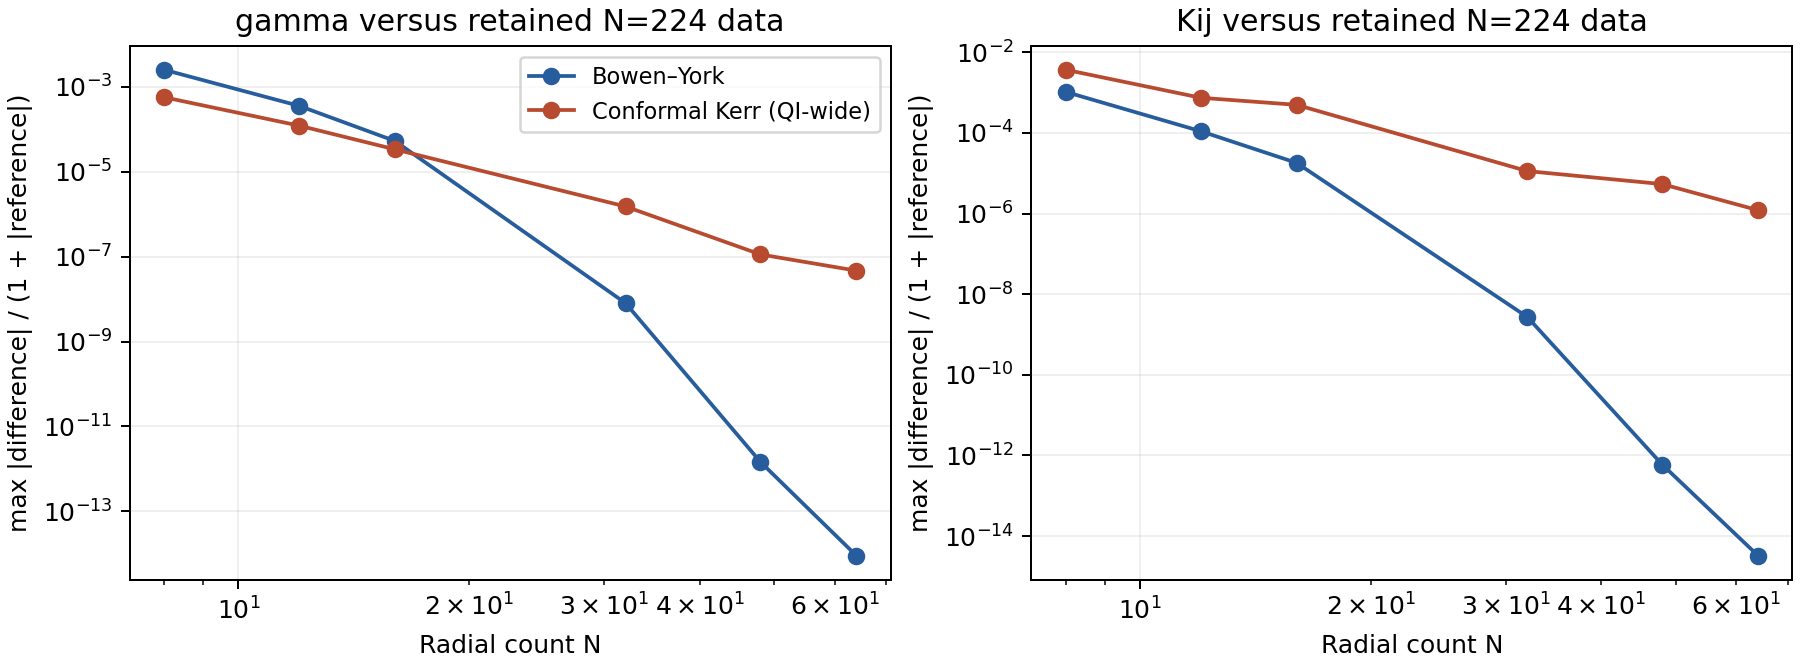
\includegraphics[width=\linewidth]{figures/binary-solutions.png}
\caption{Solution differences at fixed physical points. The continuum
formulation stays fixed within each sequence. Lower-grid convergence does
not replace the failed high-grid physical constraint gate.}
\end{figure}

The Ansorg--Br\"ugmann--Tichy convergence benchmarks use single-hole
$S/m^2=0.2$ or $P/m=0.2$, and binary $m_+=m_-=b=1$,
$P_+^y=-P_-^y=0.2$. We retain these parameters and compare
$U=u/(A-1)$ against fine references, including infinity and punctures.
The spinning single BY relative error reaches $2.31\times10^{-12}$ at16
and then roundoff; the boosted case has observed order3.976 over10/16/24/32.
Reference orders are50/70, as in the paper. The direct solver uses angular
Legendre collocation instead of theta-Chebyshev. The binary reference is
72/72/36 rather than70/70/35 to preserve even Fourier counts.
Its BY stopping gate fails at $7.95\times10^{-11}$ for a requested
$10^{-12}$, although physical fields agree with48 to near machine precision.
This diagnostic reference is not relabeled converged. No precise sixth-order
binary fit, historical BAM multigrid reproduction, or test-mass binding-energy
reproduction is claimed. Kerr counterparts use their own specified free data;
exact isolated Kerr/boosted Schwarzschild have zero elliptic correction and
are tested by convergence of their represented physical tensors.

The new optional CPU path has $r=(m/2)A/(1-A)$, Chebyshev radial roots,
Gauss--Legendre polar nodes, and no inactive second focus. The BY equation
is solved with a separated flat-operator preconditioner. Physical single-hole
fields agree with the unchanged native binary-map solver to
$1.10\times10^{-15}$ for spin and $1.10\times10^{-12}$ for boost at the stated
points. Native binary defaults and equations are unchanged.

For Liu $\chi=0.9999$, grids64/32,96/32,192/32 converge against exact geometry
on14 fixed points spanning both sides of the horizon. Finest scaled metric
and $K_{ij}$ errors are $1.60\times10^{-13}$ and $2.98\times10^{-12}$.
Independent H/M RMS reach $1.31\times10^{-8}/6.87\times10^{-10}$,
matching the exact-seed observer floors. Known-sphere horizon integration
recovers mass and spin to roundoff, with expansion RMS below $7\times10^{-13}$.
The coordinate radius is $0.25353544551648M$.
An independent radial pullback agrees to $7.90\times10^{-14}$; a necessary
FD4 step refinement0.002/0.001/0.0005 passes the unchanged vacuum bound.
These are analytic-seed and representation controls, not an AthenaK
$\chi=0.9999$ horizon-finder or time-evolution qualification.

\begin{figure}[htbp]
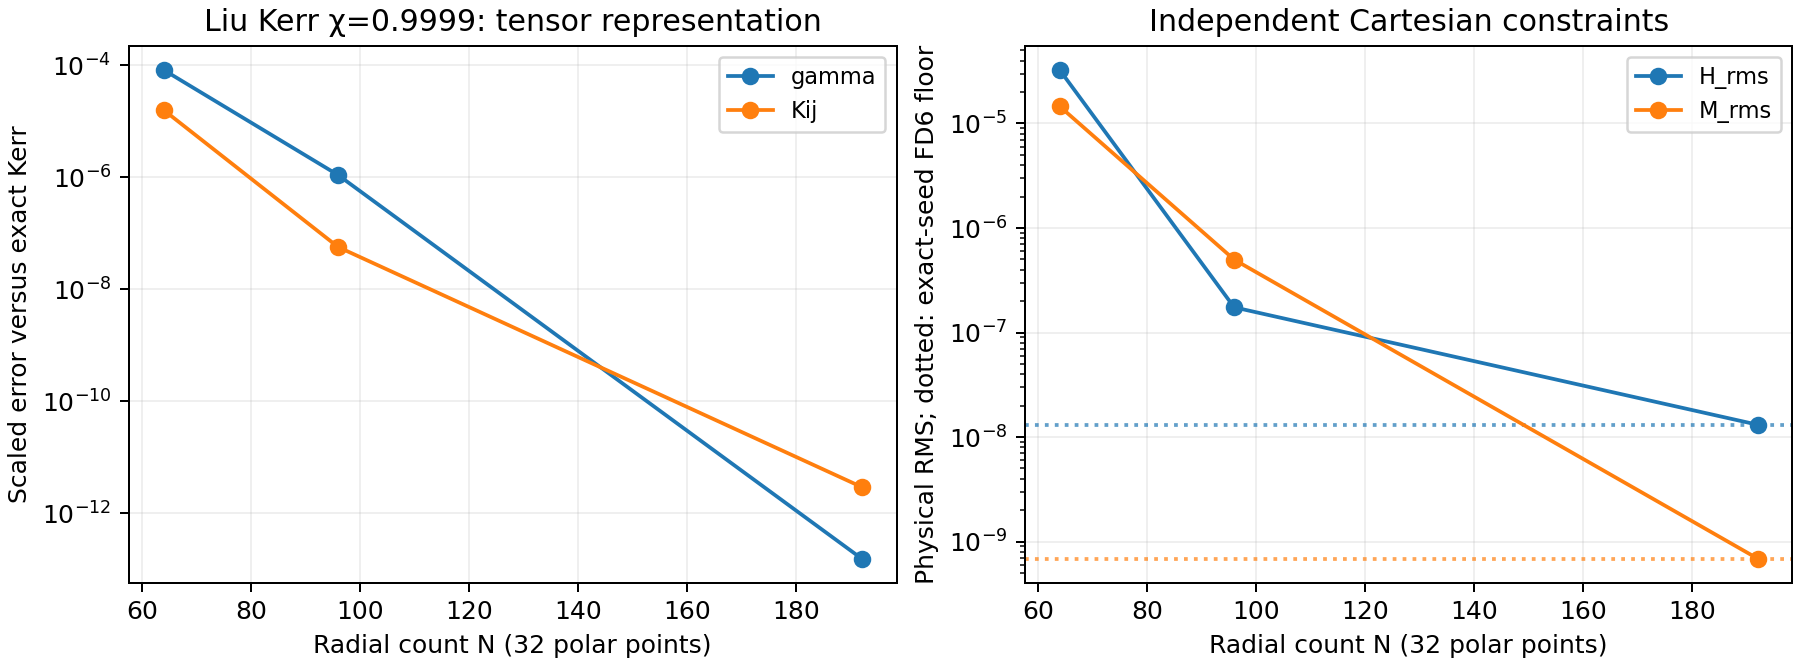
\includegraphics[width=\linewidth]{figures/liu-9999-convergence.png}
\caption{Liu $\chi=0.9999$ tensor and independent constraint convergence.
Dotted lines are exact-seed finite-difference observer floors.}
\end{figure}

A single spectral shell is suitable in principle for linear perturbations,
but evolution requires its own hyperbolic formulation and boundary treatment.
Horizon-penetrating excision and either a finite outer boundary or a
hyperboloidal asymptotic layer are separate choices. The current Liu wormhole
slice and compactification to spatial infinity are not an evolution scheme.
The new stationary Kerr free-data path below supplies nonaxisymmetric initial data; evolution remains separate work.
For related hyperboloidal constructions see
\href{https://arxiv.org/abs/0906.3342}{Zenginoglu and Tiglio (2009)}.
Selected evidence and all figures are under
\path{validation/trumpet/lower-resolution/}; large saved unknowns remain on
Perlmutter. Native solves used one shared A100; the small spherical problems
used CPU NumPy/SciPy. There was no backend benchmark sweep.

\section{Metric and time-derivative free data}
The existing four-field CTT system now accepts a physical metric perturbation
$h_{ij}$ and its fixed-Cartesian-coordinate derivative $\dot h_{ij}$ about one
stationary QI or Liu Kerr seed. The elliptic equations, Jacobian, modal
preconditioner and CUDA solve are reused. Geometry setup uses the qualified
host long-double path. With the reference Kerr lapse $\alpha_0$, shift
$\beta_0^i$ and time-independent conformal factor $\psi_0$ held fixed, define
\begin{align}
 \gamma^{\rm free}_{ij}&=\gamma^0_{ij}+h_{ij},\\
 K^{\rm free}_{ij}&=K^0_{ij}
   -\frac{\dot h_{ij}-({\cal L}_{\beta_0}h)_{ij}}{2\alpha_0},\\
 \widetilde\gamma_{ij}&=\gamma^{\rm free}_{ij}/\psi_0^4,\qquad
 K=\gamma_{{\rm free}}^{ij}K^{\rm free}_{ij},\\
 \widetilde M_{ij}&=\psi_0^2\left(K^{\rm free}_{ij}
                          -\tfrac13\gamma^{\rm free}_{ij}K\right).
\end{align}
The trace uses the full perturbed inverse metric. Its curvature, source
divergence and derivatives are recomputed; exact-vacuum Kerr identities are
used only in the unperturbed region. This is a CTT projection with prescribed
gauge, rather than a lapse/shift solve. In particular the supplied time
derivative describes the trial free data: projection can change the physical
metric time derivative reconstructed from the final $(\gamma,K)$.

A per-context callback supplies symmetric Cartesian jets of $(h,\dot h)$.
A native rotating electric $\ell=m=2$ packet ports the corrected seed from
SpEC commit \path{6b55d93e51076dc75a006837e808f1182549bf64}.
It uses a pole-regular Cartesian tensor projection and analytic second-order
jets, including the fixed-coordinate time derivative. A stationary smooth
cutoff makes the perturbation exactly zero near the throat. The native Kerr
extrinsic curvature is retained there, avoiding division by its zero lapse.
The implementation currently accepts one unboosted active hole, uses the
existing three-dimensional two-focus map with the second hole disabled, and
keeps a full three-dimensional correction. A new spherical evolution grid,
boosted free-data gauge, arbitrary multipolar packet generator and scalar
field are not implemented by this change.

Portable packet checkpoints have explicit version~3 metadata and can be
reconstructed by the corresponding AthenaK reader. Unmarked export of an
arbitrary callback is rejected; an application must retain its own provider.
Zero-amplitude recovery, independent seed/gauge oracles, a Jacobian check and
one fixed physical constraint sequence are the focused validation set.
No superradiant evolution or amplification measurement is implied.

The fixed validation packet has $M=1$, seed $\chi=0.9$, amplitude
$10^{-3}$, $\Omega=0.5$, one cycle, $r_0=6$, and cutoff radii $(2,4)$.
Both cross/far attenuation are disabled; the interior operator transition
is $(0.1,0.2)$. Only the inactive focus is moved from $z=-2$ to $z=-12$ to
resolve the exterior packet more economically. Since that hole has zero
mass, this changes the coordinate grid, not the physical free data or
constraint equations. All three accepted study levels use the latter grid.
Independent FD6 Cartesian constraints use the same 30 exterior points at
radii $0.5$--$20$ with steps $\min(0.005,0.006r)$. These are unweighted
point RMS values, not spatial-volume norms or the native stopping norm.
\begin{center}
\begin{tabular}{rrrrr}
\toprule
$N_r\times N_\theta\times N_\phi$ & $\|H\|_{\rm RMS}$ &
$\|M\|_{\rm RMS}$ & Newton/Krylov & solve (s)\\
\midrule
$48\times96\times16$ & $2.2484\,10^{-7}$ & $1.1925\,10^{-6}$ & 3/27 & 0.425\\
$64\times128\times16$ & $1.2553\,10^{-7}$ & $1.1422\,10^{-6}$ & 3/27 & 1.048\\
$96\times192\times16$ & $4.0040\,10^{-8}$ & $5.2239\,10^{-7}$ & 3/28 & 2.869\\
\bottomrule
\end{tabular}
\end{center}
At matching $N_r=96$, moving the inactive focus reduces Hamiltonian and
momentum RMS by factors $57.6$ and $10.5$. Host geometry setup at the finest
level takes $23.7$ seconds and the recorded setup/solve/observer workflow
$36.3$ seconds; the solve-only column does not describe total cost.
The unsolved packet has RMS $(8.5884\,10^{-6},1.3546\,10^{-5})$, so projection
reduces the finest norms by factors $214$ and $25.9$. The exact-seed observer
floors are $9.48\,10^{-11}$ and $1.28\,10^{-12}$.
The finest pointwise maxima are $1.04\,10^{-7}$ and $1.19\,10^{-6}$;
this initial-data demonstration remains labeled preliminary.

The native packet matches an independent spherical-basis implementation of
the cited SpEC seed within $4.4\,10^{-19}$ absolute error, including poles and
both propagation/handedness signs. Zero amplitude recovers the unperturbed
sampler and residual bit for bit. Independent fixed-coordinate time,
ADM gauge-map and Jacobian checks pass. At $r=10$, the physical metric's
$\ell=m=2$ tensor projection survives the solve; its amplitude changes by
about $0.023\%$, while the reconstructed time derivative's amplitude changes
by about $13\%$. These are metric multipoles, not Weyl scalars or an energy
flux. A more precise incoming-wave/scattering study must analyze the final
radiative data rather than assume the trial time derivative is unchanged.
\begin{figure}[htbp]
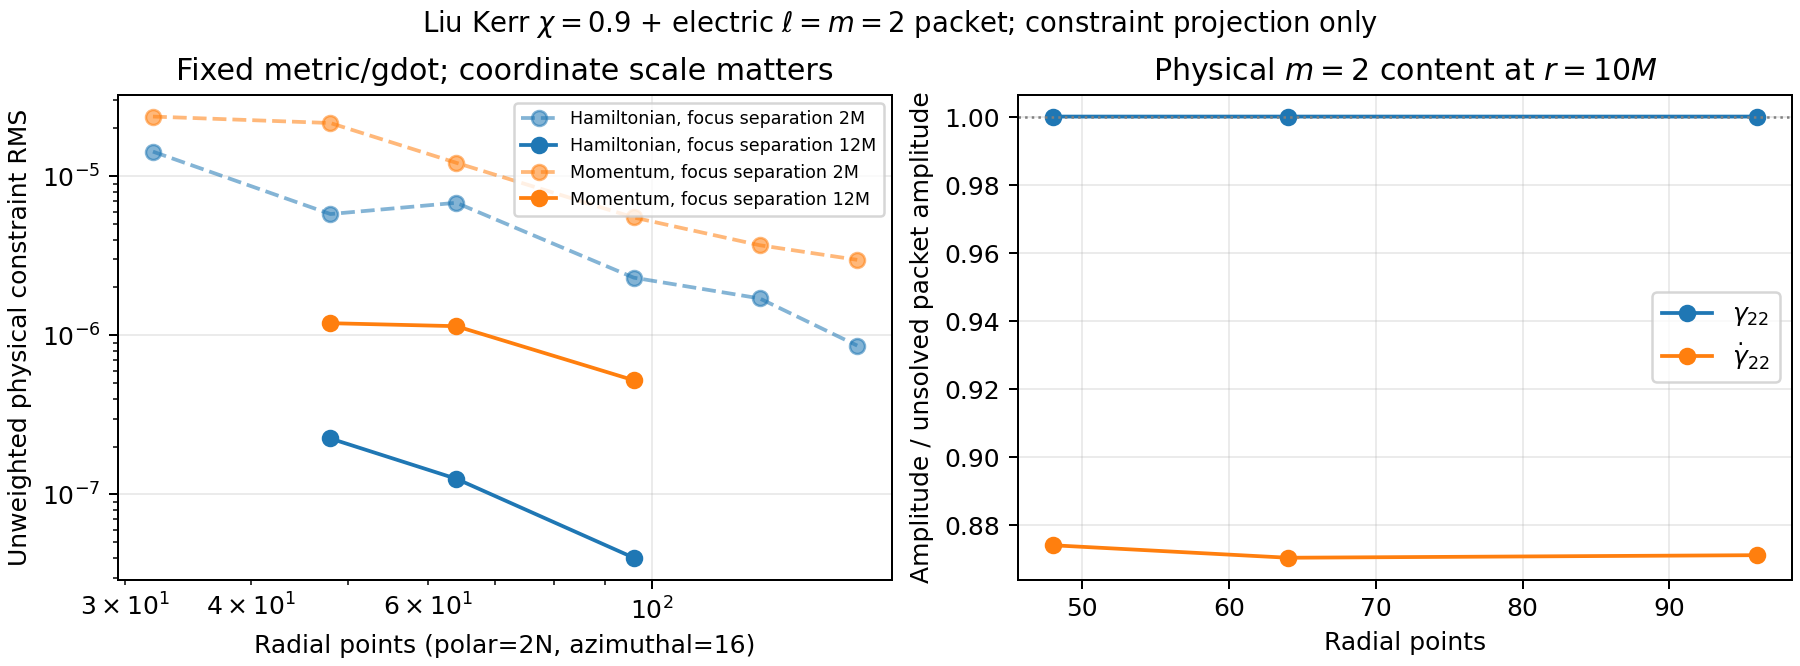
\includegraphics[width=\linewidth]{figures/wave22-convergence.png}
\caption{One fixed Liu Kerr plus electric packet. Dashed curves retain the
underresolved smaller-coordinate-scale results. Solid curves use one fixed
larger scale at three resolutions. The right panel shows physical tensor
multipoles before/after constraint projection, without an evolution claim.}
\end{figure}

The exported finest solution passes a separate-process producer/CPU-reader
comparison at 1,602 points, including the packet, throat and trial horizon
regions: all nine exported fields, including metric derivatives, agree bit
for bit. AthenaK then imports the same version~3 checkpoint and runs its
horizon finder with $\ell_{\max}=8,12,16$ and a final angular-quadrature increase
from 32 to 48. All searches pass the unchanged $10^{-7}$ expansion-RMS bound
and enclose the modified interior ball. The final measurements are
\[
 A_H=36.08785490004055,\quad M_{\rm irr}=0.84731638814292,\quad
 M_H=1.00000003473985,\quad \chi_{\rm coord}=0.89999993746827.
\]
Here $M_H$ is the Christodoulou mass from the measured area and coordinate
rotation integral, not the total ADM mass of the wave-containing spacetime.
The final expansion RMS is $7.34\,10^{-8}$. Coordinate spin is not an
approximate-Killing-vector measurement for this nonaxisymmetric geometry.
This is an actual finder search of solved perturbed data, rather than an
integral on an assumed analytic sphere. The mesh import/evolution limit is
zero time steps; no superradiant amplification or perturbed
$\chi=0.9999$ validation is claimed.

An additional deliberately incompatible warm start adds constants to the
auxiliary nodal $P$ fields. It violates the homogeneous focus rows (a constant
$m=0$ mode has a nonzero $-(m+1)P$ focus term) and fails Krylov convergence.
The failed diagnostic is retained as \path{wave22/incompatible-start.json}.
Arbitrary correction guesses are therefore not qualified; use the default
zero correction, a compatible prolongation, or a guess satisfying the
axis/focus conditions. This limitation is distinct from perturbing the
physical free metric and its time derivative.

A compatible nonzero start, $1.05$ times the saved correction, converges
in two Newton and 17 Krylov iterations to the same sampled physical metric
and extrinsic curvature within $7.6\,10^{-14}$. The auxiliary nodal-$P$
maximum difference is $7.8\,10^{-7}$, so this is physical-field agreement at
the declared observers, not bitwise equality of all auxiliary coefficients.
Halving the independent FD6 steps changes pointwise Hamiltonian values by
at most $1.15\,10^{-9}$ and momentum components by $1.40\,10^{-12}$, below
the reported constraint errors. The complete evidence and one compact plot
are retained under \path{validation/trumpet/wave22/}.

\section{Reproducibility and remaining work}
The native and consumer branches are \path{codex/hispid-trumpet} and
\path{codex/hispid-trumpet-pgen}; neither is merged. Detailed evidence, failed
attempts, hashes and executable identities are under \path{validation/trumpet/},
with the audit trail in \path{docs/TRUMPET_IMPLEMENTATION.md}. Key records are
\path{convergence/assessment.json}, \path{spin-focused-map/horizon160-warm/},
\path{affine-horizon/exact/horizons-v4/}, and \path{axisymmetric/radial-comparison.json}.
Commands are retained beside each run. The original performance report is
preserved without extending its campaign.

Completion still requires an accepted moderate physical-convergence sequence,
resolution of the extreme binary constraint errors, qualified boost-binary
horizon measurements and measured-$M_{\rm irr}$ separation calibration, followed
by a final evidence audit. Pending runs and failed gates are not counted as
validation. This report is an interim snapshot, not completion of the goal.

\smallskip\noindent References:
\href{https://arxiv.org/abs/1409.1887}{Dennison--Baumgarte--Montero (2014)};
\href{https://arxiv.org/abs/1410.8607}{Ruchlin et al., high-spin/high-boost puncture data};
\href{https://arxiv.org/abs/1806.08364}{boosted trumpet construction reference}.
\end{document}
